%!TEX root = ../report.tex
\chapter{Introduction}
The objective of this project is to learn a general similarity function for sonar image patches, which is able to predict that two input sonar image patches contain different views of a same object or not. 
But instead of using hand designed features (such as SIFT) we will explore different deep learning architectures to encode such a function. The state of the art results were achieved by Matias et al. \cite{stateoftheart}
This implementation of deep learning in sonar image patch matching was one of the first. It is influenced by work of Zagoruyko et al. \cite{zagoruyko2015learning}.
\subsection{Data}
The dataset for this thesis is obtained from Matias' PhD project \cite{stateoftheart}, it consists of images from nine different object types which are common marine debris. 
The object types are metal cans, bottles, drink carton, metal chain, propeller, tire, hook, valve. In \cite{stateoftheart}, in controlled underwater environment total of 2072 images; 
that is about 2500 instances of the aforementioned object types were captured using forward looking sonar. As part of the same work \cite{stateoftheart}, matching and non-matching pairs 
of sonar image patches were generated using a patch generation algorithm where each patch were obtained from meaningful crops of the original sonar images. 
Authors have figured that 96x96 pixels is the best size of the crops.

\begin{figure}[ht]
\centering
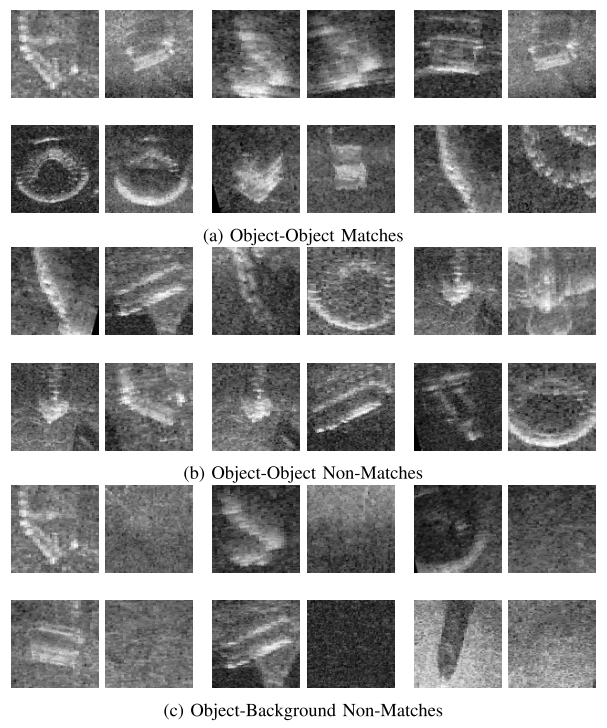
\includegraphics[height= 8cm]{images/contrastive/generated_patches}%TODO exchange this with the actual latex code
\caption{Some sample of the matching and non-matching pairs }%generated by Matias et. al \cite{stateoftheart}}
\label{fig:generated_patches}
\end{figure}

To create matching pair, two patches that belong to the same object-type but different perspective and insonification level were used. For generating non-matching pair, two instances of different 
object-types were used. Also, one instance of an object and a background patch, which contains no object instance, were used to generate additional non-matching patches. According to the work \cite{stateoftheart}, 
for balanced and effective learning, the ratio of matching and non-matching pairs in both train and test data is maintained 1:1. That is, for every ten matching pair five object-object non-matching 
and five object-background non-matching pairs were generated. Using the patch generation algorithm total of 39840 pairs were generated from the instances of 6 distinct object type, which were used as the train data.
While another 7440 pairs were generated from the instances of remaining object types, for testing purpose. This test dataset does not contain any common object with the training dataset,
it should be a good test for the generalization of the approaches. The labels for the data are 0 and 1 representing non-matching and matching pairs respectively. 
For this thesis the previously described datasets generated in \cite{stateoftheart} will be used.
All pairs of patches are supplied in form of tensors \cite{tensors}, each of shape (2,96,96), in HDF5 files.

\chapter{Evaluation and results}
\section{Contrastive loss}
Using contrastive loss higher dimensional input data (e.g. pair of images) can be mapped in the much lower dimensional output manifold, where similar pairs are placed closer to each other and 
the dissimilar pairs have bigger distances between them depending on their dissimilarity.  So using this loss function the “distance” between two input patches projected in the output manifold can be 
predicted and if the distance is closer to 0 then the input pairs are matching, otherwise its dissimilar(more than 0.5). The formula for the loss is shown below. 
\begin{figure}[ht]
\centering
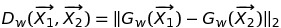
\includegraphics[height= 0.45cm]{images/contrastive/contrastive_loss_formula1.jpg}%TODO exchange this with the actual latex code
%\caption{Contrastive loss}
\label{fig:contrastive_loss_formula1}
\end{figure}

\begin{figure}[ht]
\centering
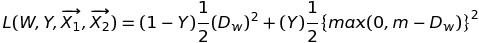
\includegraphics[height= 0.7cm]{images/contrastive/contrastive_loss_formula2.jpg}
%\caption{Conv2D filters analysis}
\label{fig:contrastive_loss_formula2}
\end{figure}

Here L is the loss term, the formula presented here is the most generalized form of the loss function, suitable for batch training. 
$ \vec{X_1}$, $ \vec{X_2}$ represents a pair of input image vectors. Y are the labels, 0 for similar pair and 1 for dissimilar pair. D\_w is the parameterized distance function to be learned by the algorithm. 
m is the margin and m is always greater than zero and it defines a radius around G\_w. The dissimilar pairs only contribute to the loss function if their distance is within the radius.
One of the idea for evaluating this loss function is to use it with a Siamese network, as the loss function takes a pair of images as input. So its very relevant to our project. 
Since this is just a loss function, different network architectures can be evaluated with it to find out the best performance overall.
%\begin{figure}[ht]
%\centering
%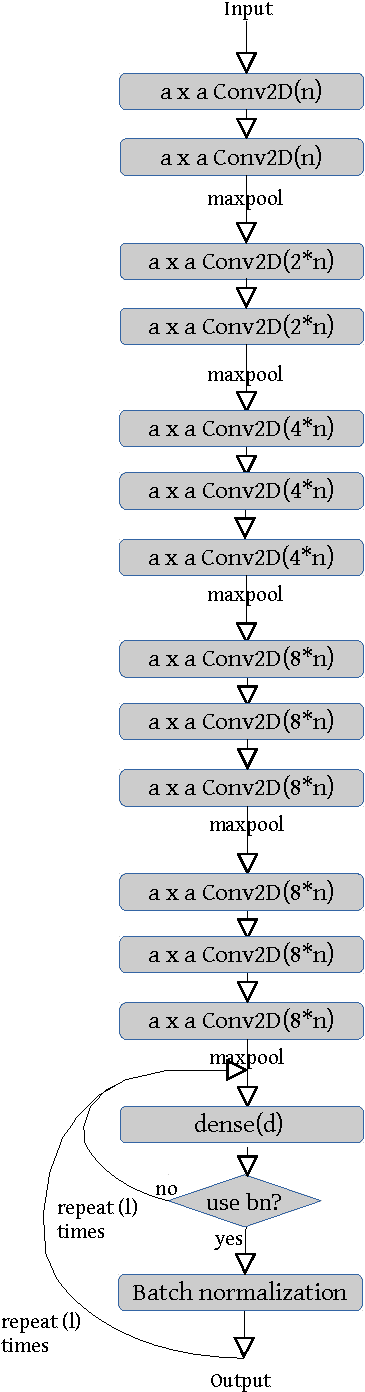
\includegraphics[height= 10cm]{images/contrastive/contrastive_loss_vgg_branch}
%\caption{VGG branch structure}
%\label{fig:contrastive_loss_vgg_branch}
%\end{figure}

%\begin{figure}[ht]
%\centering
%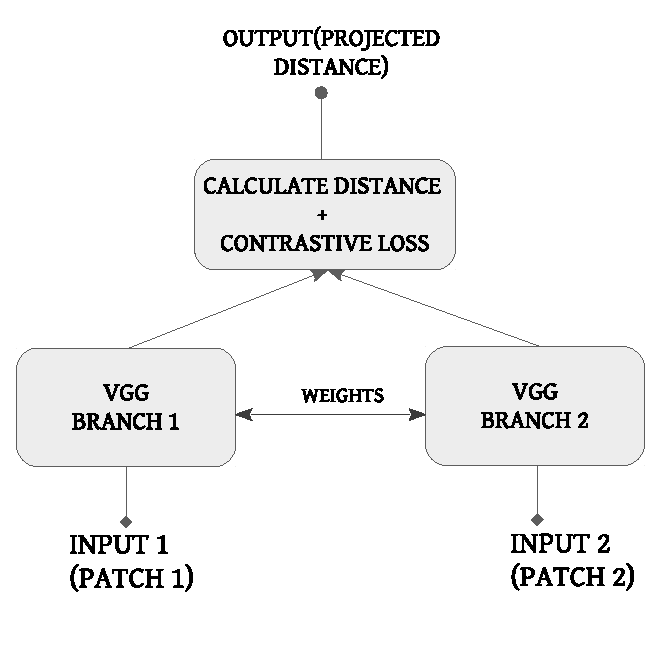
\includegraphics[height= 6cm]{images/contrastive/siamese_contrastive_loss}
%\caption{VGG siamese network with contrastive loss}
%\label{fig:siamese_contrastive_loss}
%\end{figure}

\begin{figure}
    \centering
    \begin{subfigure}[b]{0.4\textwidth}
        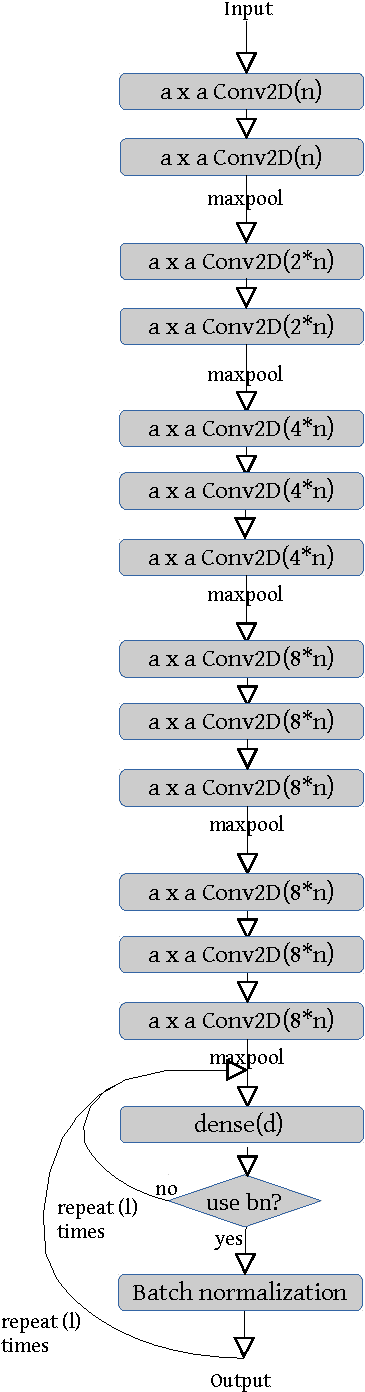
\includegraphics[height= 10cm]{images/contrastive/contrastive_loss_vgg_branch}
	\caption{VGG branch structure}
	\label{fig:contrastive_loss_vgg_branch}
    \end{subfigure}
    ~ %add desired spacing between images, e. g. ~, \quad, \qquad, \hfill etc. 
      %(or a blank line to force the subfigure onto a new line)
    \begin{subfigure}[b]{0.4\textwidth}
        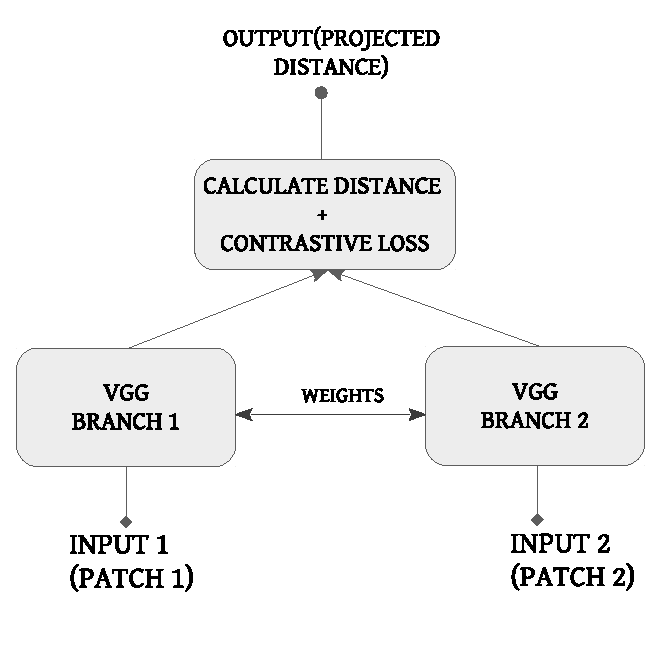
\includegraphics[height= 6cm]{images/contrastive/siamese_contrastive_loss}
        \caption{VGG Siamese network with contrastive loss}
        \label{fig:siamese_contrastive_loss}
    \end{subfigure}    
    \caption{Network structure}\label{fig:network_structure_vgg_siamese}
\end{figure}

%TODOExplain that the vgg structure is used as the branch of the network
%TODOIs it used as the feature extraction network, any scientific litrature on this?
\subsection{Best hyper-parameters search spaces}
 %How do we know that this script implementation is right? Perhaps check it with a bench mark data set 
 The hyper parameters of the network are as follows.
  \begin{enumerate}
   \item Conv2D filters(n) 
   \item Kernel size(a)
   \item Layers (single, two, three)(l) n,a,l this variables are depicted in figure \ref{fig:contrastive_loss_vgg_branch}
   \item Initializers ( He\_normal, He\_uniform, Glorot\_uniform(default), Glorot\_normal(Also called Xavier normal) RandomNormal.    
   \item Dense filters (32, 64, 96, 256, 512, 1024, 2048)
   \item Dropouts (0.1, 0.2, 0.3, 0.4, 0.5, 0.6, 0.7, 0.8)
   \item Batch normalization (True or False)
   \item Batch Size (32, 64, 128, 256, 512)
   \item Optimizer ( Adam, Nadam, Adadelta, Adamax, RMSprop)
   \item Learning rate (0.01, 0.007, 0.005, 0.002, 0.0007, 0.0005, 0.0002, 0.0001, 0.00007, 0.00005, 0.00002, 0.00001)   
  \end{enumerate}

In the above section the hyper parameters and the search space has been displayed.
  
\subsection{Analysis}
Since contrastive loss returns projected distance, here close to zero means similarity and 1 means dissimilarity. Our original data is 1 means similarity between patches.
Hence the labels for train, validation and test data here are all flipped. ( new\_label = 1 - old\_label )

Overall search space is divided into smaller parts and been evaluated with a common starting network configuration, that we found to be working good after some manual tuning and many trials.

\subsubsection{Training process}
The train data has been divided into train and validation data randomly using sklearn train test data split \cite{sklearnsplit} in 8:2 ratio. But please note that the roles of the validation data in keras 
is different than classic training method. In keras the validation data is not used to update the weights. Instead this validation dataset can be used to monitor the network performance in terms of 
validation accuracy and validation loss. Using callback functions such as EarlyStopping and ReduceLROnPlateu \cite{kerascallbacks} the network validation performance can be monitored after each epochs.
By configuring the callbacks properly the training can be stopped if the validation accuracy or loss does not improve after a number of epochs (parameter name EarlyStopping patience) the training process terminates.
Similarly, if the validation performance does not improve after some epochs the learning rate can be reduced by a previously determined factor using ReduceLROnPlateu to come out of the local minima. The patience values 
are set after some manual trials.
\subsubsection{Conv2D filters analysis}
The 'filters'\cite{kerasconv} defines the number of output filters in each convolution layers. Now for all the 13 convolution layers in the network the filters size can be easily calculated from the first filter size. In figure
\ref{fig:contrastive_loss_vgg_branch} it has been shown that the filters for the Conv2D layers are n, n, 2n, 2n, 4n, 4n, 4n, 8n, 8n, 8n, 8n, 8n, 8n respectively. Here 4n means 4 times n obviously. 
\begin{figure}[ht]
\centering
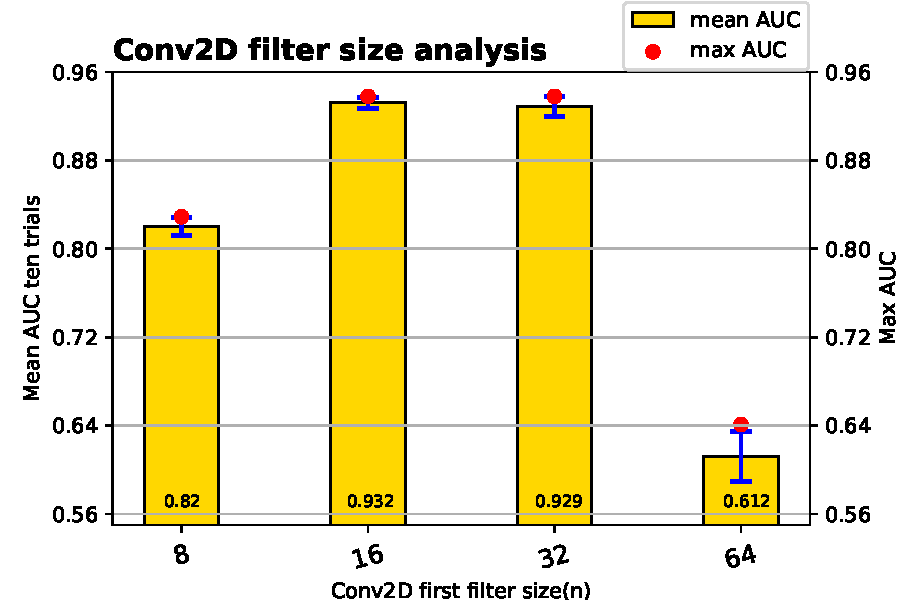
\includegraphics[height= 5cm]{images/contrastive/contrastive_loss_con2d_filter_bar}
\caption{Conv2D filters analysis}
\label{fig:contrastive_loss_con2d_filter_bar}
\end{figure}

So for the best performing \ref{fig:contrastive_loss_con2d_filter_bar} network is having the Conv2D filters as follows, 16, 16, 32, 32, 64, 64, 64, 128, 128, 128, 128, 128, 128.  

\subsubsection{Kernel size analysis}
The kernel size parameter defines the height and width of the 2 dimensional convolution window for all the Conv2D layers in the VGG network. table \ref{table:kernel_size} it is clear that the kernel size 3 
works so much better than 5 and 7 kernel size. 

\begin{center}
    \begin{tabular}{||c c c||} 
      \hline\hline
      Rank & Kernel size & Mean AUC (10 trials) \\[0.5ex] 
      \hline
      1 & 3 &  0.932\\      
      \hline
      2 & 5 &  0.799\\      
      \hline
      3 & 7 &  0.481\\      
      \hline
    \end{tabular}
  %\caption{Kernel size analysis}
  \label{table:kernel_size}
\end{center}

\subsubsection{Dense units size analysis} 
The specified 'units' (d) in figure \ref{fig:contrastive_loss_vgg_branch} determine the output size for a dense layer. Seems like single dense layer (l) in figure \ref{fig:contrastive_loss_vgg_branch} works best. But performance 
of two layers are also not so bad.
128 and 2048 has been included for the final grid search since they have the best results. Although conceptually this is bit unexpected to see both points close to the two extremes works best, usually it should have been few points 
in the middle of the search space or near just one boundary but not both. %TODOMight have to do the search for 4096.

\begin{figure}[ht]
\centering
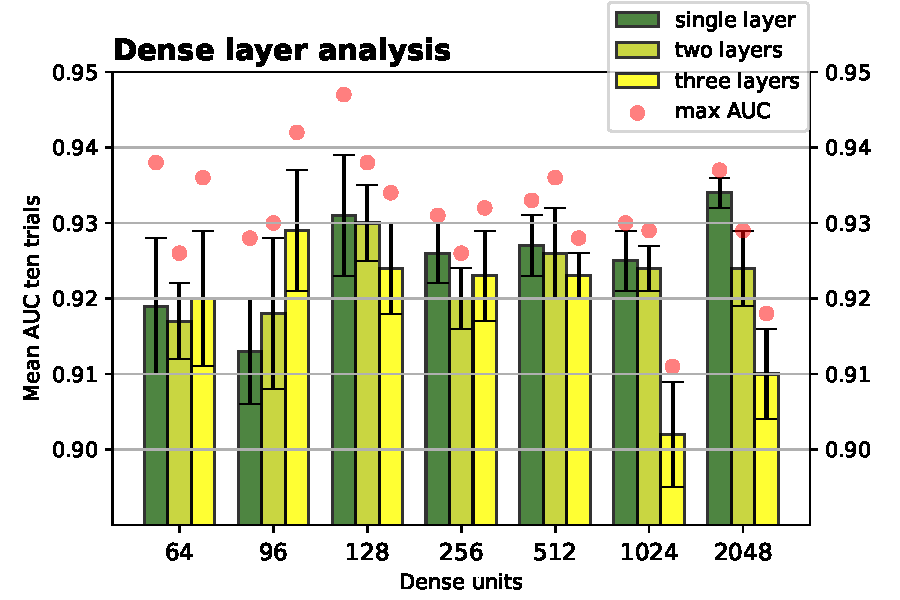
\includegraphics[height= 6cm]{images/contrastive/contrastive_loss_dense_bar}
\caption{Dense units and layers analysis}
\label{fig:contrastive_loss_dense_bar}
\end{figure}

\subsubsection{Initializer}
Keras initializers\cite{kerasinit} control/define the way the initial random weights in keras layers are set.

%Add the formulas in math format.
%Add what is tensor ?
\textbf{Zeros} : This is one of the simplest of the initializers. It generates tensors initialized to 0.\\
Instantiation: keras.initializers.Zeros()

\textbf{RandomNormal} : This Initializer uses normal distribution to generate the tensors.\\
Instantiation: keras.initializers.RandomNormal(mean=0.0, stddev=0.05, seed=None)

\textbf{RandomUniform} : This Initializer uses uniform distribution to generate the tensors.\\
Instantiation: keras.initializers.RandomUniform(minval=-0.05, maxval=0.05,\\
 seed=None)

\textbf{Glorot\_normal} : Glorot normal initializer is also known as Xavier normal initializer. It generates samples from a truncated normal distribution which is centered at 0 with  
standard deviation (stddev) = sqrt(2 / (fan\_in + fan\_out)) where fan\_in represents number of input units in the weight tensor and the number of output units in the weight tensor is the fan\_out.\\
Instantiation: keras.initializers.glorot\_normal(seed=None)

\textbf{Glorot\_uniform} : Glorot uniform initializer, also called Xavier uniform initializer. It draws samples from a uniform distribution within [-limit, limit] 
where limit is sqrt(6 / (fan\_in + fan\_out)) where fan\_in represents number of input units in the weight tensor and the number of output units in the weight tensor is the fan\_out.\\
Instantiation: keras.initializers.glorot\_uniform(seed=None)

\textbf{He\_normal} : It draws samples from a truncated normal distribution centered on 0 with standard deviation (stddev) = sqrt(2 / fan\_in) where  fan\_in represents the number of 
input units in the weight tensor.\\
Instantiation: keras.initializers.he\_normal(seed=None)

\textbf{He\_uniform} : He uniform variance scaling initializer draws samples from a uniform distribution within [-limit, limit]. Here, limit is sqrt(6 / fan\_in) and fan\_in represents the number
of input units to the weight tensor.\\
Instantiation: keras.initializers.he\_uniform(seed=None)

\begin{itemize}
 \item The initializers evaluated here are in two different sets. Kernel initializers for the convolution networks and kernel initializers for the Dense layers. 
 \item The kernel initializers evaluated for the convolution layers (Conv2D) are He normal and uniform, Glorot normal and uniform and RandomNormal. 
 \item Initializer for Conv2D and dense layer. It is found out that the RandomUniform (default settings) is not converging at all for Conv2D initializer. 
 \item For the Dense layers He normal and uniform and Glorot normal and uniform is used
 \item The bias initializer, for both Conv2D and Dense layers, is used with default 'Zeros' option. %why ??
 \item In keras for both Conv2D and Dense the default kernel initializer is Glorot uniform
 \item Popular Intuition is that Glorot or Xavier initialization works better with Sigmoid, while He uniform/normal works better with Relu.
 \item In our case there are 13 Conv2D layers compared to only one or two dense layers, so the Conv2D initializer is expected to have more effect.
 \item All the initializers used with seed None. Because we did not know which seed value to provide for the best result.

\end{itemize}

%details on the choice of the initializer
%add sources/references

%can we add the maximum points in the 3D graph?
\begin{figure}[ht]
\centering
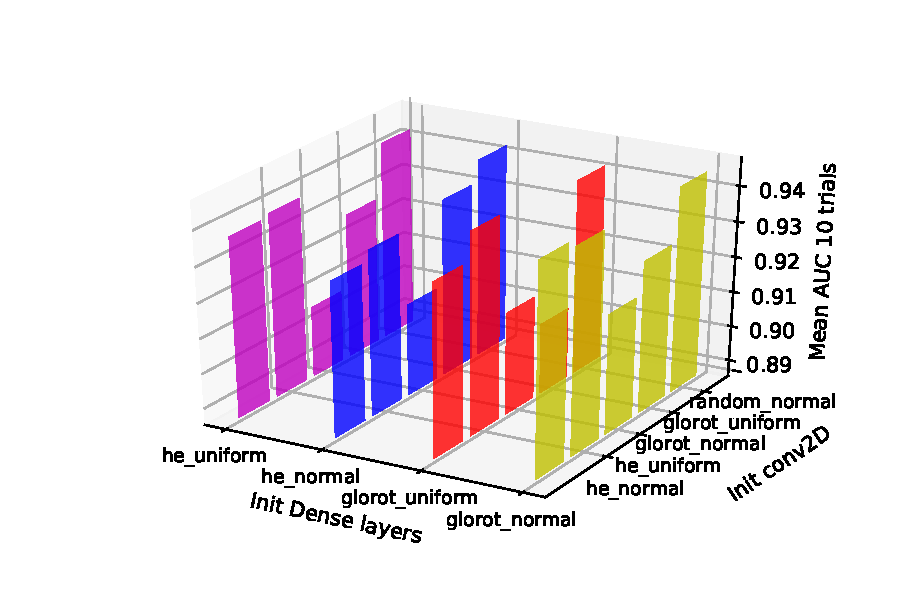
\includegraphics[height= 8cm]{images/contrastive/3DbarGraph}
\caption{Comparison of initialization of Conv2D and Dense layers}
\label{fig:3DbarGraph_initialization}
\end{figure}
In this graph, observed mean AUC is reported for different combination of Conv2D initializer and Dense Initializer. The x axis of the graph represents dense layer initializer 
and the y axis represents the Conv2D initializer. In the z axis the mean AUC of ten trials is shown. Please note that the z-axis values are clipped and starts from 0.89. This is 
to be able to show the bar heights differences effectively. Otherwise, if the bars were plotted from zeros they all look similar height as the values are very close indeed.
Lowest mean AUC value obtained is 0.903 and the highest is 0.943. The bar chart starting value selected in such a way that all the bars are clearly visible and comparable.
Now the Interesting observations from the graph are as follows.

\begin{itemize}
 \item The performance of RandomNormal as the initializer for Conv2D layers over all good.
 \item Performance of the Glorot normal and uniform both as Conv2D initializer is comparatively worse than others.
 \item Performance of He initializers are over all quite good as a Conv2D initializer. 
 \item As the Dense layer initializer glorot normal is found to have performed the best.
 \item Over all performance wise the He normal as the Conv2D and glorot normal as the dense Initializer has performed slightly better 0.943 than second best 0.941 with 
 (He uniform, Glorot normal), and also (RandomNormal, Glorot normal) both. The best mean AUC results are shown below.  
 \item From table \ref{table:kernel_init} it is observed that there might be a trend that with RandomNormal kernel initializers, the standard deviation is very low, but the 
 max AUC values are consistently lower than the He counter parts. However all the top ranking results are very close in terms of mean AUC.
\end{itemize}

\begin{center}
  \begin{table}
    \begin{tabular}{||c c c c c c||} 
      \hline\hline
      Rank & Init Conv2D & Init Dense & Mean AUC & STD & MAX AUC\\ [0.5ex] 
      \hline
      1 & He normal & Glorot normal & 0.943 & 0.007 & 0.953 \\ 
      \hline
      2 & He uniform & Glorot normal & 0.941 & 0.012 & 0.961 \\
      \hline
      3 & RandomNormal & Glorot normal & 0.941 & 0.004 & 0.946 \\
      \hline
      4 & He uniform & Glorot uniform & 0.94 & 0.008 & 0.952\\
      \hline
      5 & RandomNormal & He normal & 0.939 & 0.005 & 0.946\\
      \hline
      6 & RandomNormal & He uniform & 0.939 & 0.005 & 0.948\\
      \hline
    \end{tabular}
  \caption{Kernel initializer top results}
  \label{table:kernel_init}
\end{table} 
\end{center}

\flushbottom
\newpage

\subsubsection{Dropouts analysis}


\begin{figure}[ht]
\centering
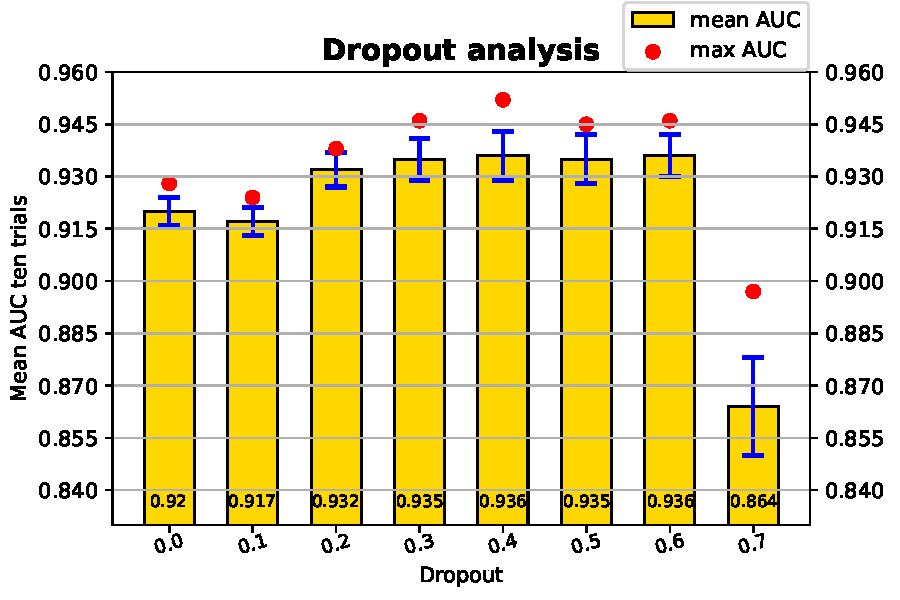
\includegraphics[height= 7cm]{images/contrastive/contrastive_loss_dropout_bar}
\caption{Dropouts analysis}
\label{fig:contrastive_loss_dropout_bar}
\end{figure}

From the figure \ref{fig:contrastive_loss_dropout_bar} it is noticeable that the performance for dropout values 0.3, 0.4, 0.5 and 0.6 are very close and the higher than with too less dropouts like 0, 0.1. Also higher
than high dropout value such as 0.7. 0.4 is chosen as the best value for the dropout, because it has highest max AUC value along with highest mean AUC. This result is very expected, based on the common findings.

\flushbottom
\newpage

\subsubsection{Batch normalization analysis}
Small batch training is better than one by one training also better than
training the whole data set all at once. Small batch training with batch normalization is advantageous because it's converges faster than doing one by one. Batch normalization reduces the need for carefully tuning the 
initial weights, also to some extend limits the need for too much of regularizers such as dropouts. Concept of batch normalization was introduced by Ioffe and Szegedy in 2015. It is influenced by the idea from Lecun1998b and 
Wiesler and Ney, 2011 that the inputs which are linearly transformed to have unit variance and zero mean. The learning rates are generally kept lower because 
an outlier might cause big effect in already learned activations. As a result of keeping the inputs normalized the outlier cases also affects the overall learning process lesser. Hence Batch normalization
should also enable the use of higher learning rates. The batch normalization layer is only applied after each fully connected or dense layer. To test it's effect we have evaluated three cases, without Batch normalization, 
with batch batch normalization, when adding the batch normalization after the dense layer but before the Activation function 'Relu'. Thirdly, after dense layer and activation 'Relu'. Mean AUC comparisons are as follows
(same epochs).
\begin{center}
    \begin{tabular}{||c c c c c||} 
      \hline\hline
      Rank & Batch normalization & Mean AUC (10 trials) & STD & Max AUC\\[0.5ex] 
      \hline
      1 & Without &  0.932 & 0.005 & 0.938\\      
      \hline
      2 & Before activation Relu & 0.9 & 0.012 & 0.926\\   
      \hline
      3 & After activation Relu &  0.874 & 0.011 & 0.893\\   
      \hline
    \end{tabular}
  %\caption{Kernel size analysis}
  \label{table:batch_normalization}
\end{center}
The findings are surprising, It has been noted during the training that the network can achieve higher training accuracy in the same number of epoch than without batch normalization. However the generalization performance on the 
test data is worse using batch normalization. May be this can be evaluated along with different batch sizes. May be also higher learning rates. %TODO May be add a time duration compare as well.

\begin{figure}[ht]
\centering
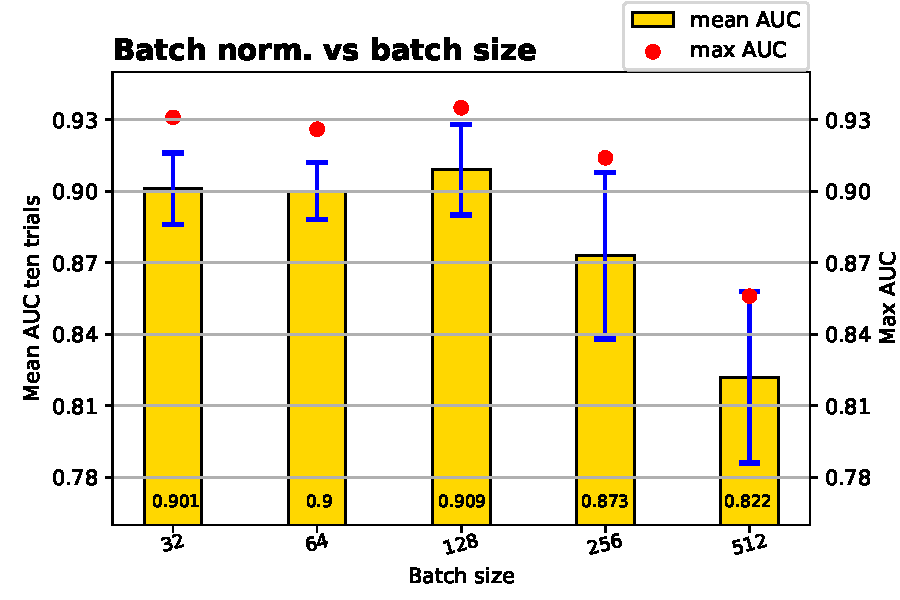
\includegraphics[height= 5cm]{images/contrastive/contrastive_loss_bnvsbs_bar}
\caption{Batch norm. vs batch size analysis}
\label{fig:contrastive_loss_bnvsbs_bar}
\end{figure}

The batch size and batch normalization correlation analysis is done in figure \ref{fig:contrastive_loss_bnvsbs_bar}. The idea was that the batch normalization performance might increase with increase in the batch size. The 
batch size is, the more it resemble the actuak distribution in across the whole data, this was one of the intuition. 

\subsubsection{Learning rate and optimizer}
%In practice, it is currently not common to see L-BFGS or similar second-order methods applied to large-scale Deep Learning and Convolutional Neural Networks. Instead, SGD variants based on (Nesterov’s) momentum are more standard because they are simpler and scale more easily.
%http://ruder.io/deep-learning-optimization-2017/index.html#understandinggeneralization useful source 
During the training, in backpropagation step the analytic gradient is computed which is used to update the parameters of the network. This update stage could be done in different ways, this is where the optimizer come
into action. While the main target of the deep learning task is to find the minima, the optimizers can control how soon or robustly the minima is found. There is a very compelling comparison of optimization process to 
a ball or particle rolling down hill in the Stanford lecture series \cite{cs231n}. It compares the loss function to a hill and randomly initializing the weights to particle with zero velocity at random points on the hill.
Now the optimization process is compared to simulating the particle's motion (parameter vector) of rolling down the hill landscape (loss).
Keras sources \cite{kerasopt} gives very brief description of the optimizers. Important optimizers are as follows.\\
\textbf{SGD} Stochastic gradient descent optimizer. The very first of it's kind, conceptualized by H. Robbins and S. Munro back in 1951. Even though it remains one of the most preferred optimizer till date 
(different variations i.e with momentum, Nesterov etc), this optimizer is not evaluated in this work in favor of more theoretically advanced optimizers. \\
\textbf{Adagrad} Instead of globally varying the learning rate, the concept of per parameter adaptive learning rate was first introduced by Duchi et al. in Adagrad optimizer. It seems it has a limitation though, 
the use of monotonic learning rate is often too aggressive and the learning stops too early. This optimizer is also not included in this study in favor of more advanced optimizers.\\
\textbf{RMSprop} RMSprop try to compensate the aggressive monotonically decreasing learning rate from Adagrad by introducing the moving average of squared gradient.\\
\textbf{Adam} Adam can be seen as RMSprop with momentum.\\
\textbf{Nadam} It incorporates Nesterov momentum into Adam.\\
\textbf{Adamax} Adamax is a variant of Adam which uses infinity norm.\\
\textbf{Adadelta} It is like Adagrad with moving window of gradient updates. \\

\textbf{Results}
It is very Interesting to note that all the optimizers were found to be working very good and the best mean AUC result for each of the optimizers are rather close. But for different learning rates. Nadam is the best performer here.
Not only the best mean AUC is highest but also the max AUC of one of the ten trials is the highest. So we are selecting Nadam for finer evaluations. Since all the results are close does not make lot sense to evaluate 
the best network for all the optimizers. 

The top results are as follows:
( Adam+0.00001, Nadam+0.0002, Adadelta+0.005, Adamax+0.0007, RMSprop+0.0002) 

\begin{figure}[ht]
\centering
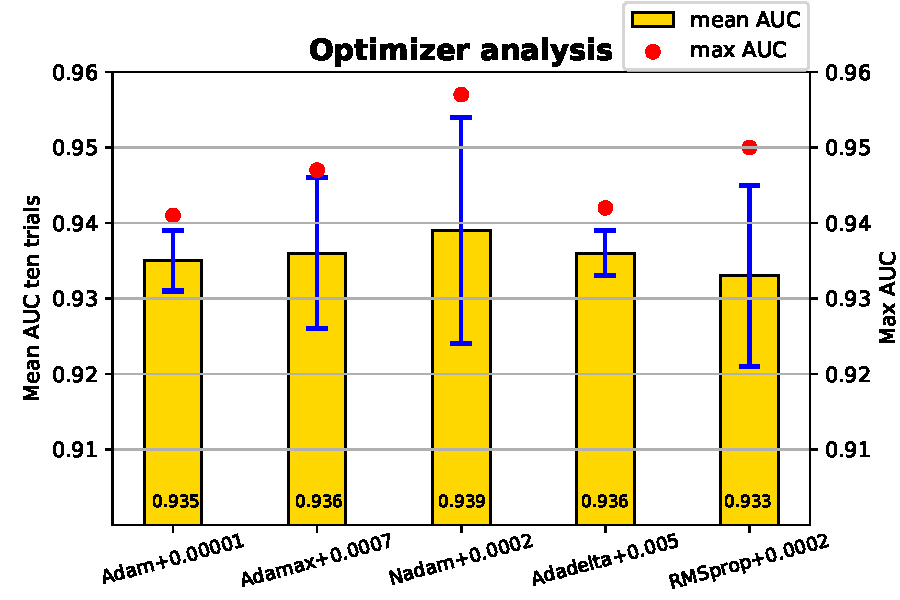
\includegraphics[height= 7cm]{images/contrastive/contrastive_loss_optimizer_bar}
\caption{Best optimizer and learning rate}
\label{fig:contrastive_loss_optimizer_bar}
\end{figure}

\subsubsection{Batch size analysis}
If the batch size is too low then it takes more time and lower than a certain size network does not train well too.If the batch size is very big then it may train faster but might converge 
to sharp minimizers of the training function. This might result in poor generalization.

\begin{figure}[ht]
\centering
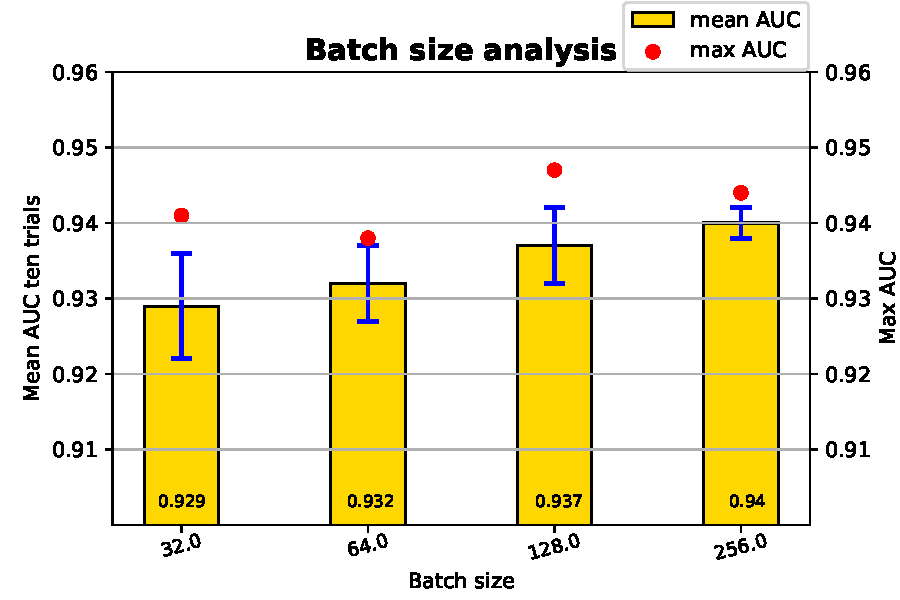
\includegraphics[height= 7cm]{images/contrastive/contrastive_loss_batchsize_bar}
\caption{Batch size analysis}
\label{fig:contrastive_loss_batchsize_bar}
\end{figure}

It is observed from the figure \ref{fig:contrastive_loss_batchsize_bar} that the test AUC somehow increases with the increase in batch size. Although it takes more epochs to reach the convergence. 
Since the 256 batch size was the boundary condition which performed the best, batch size 512 was also evaluated. But it does not train well and the validation accuracy remains stuck near 50\%.
hence batch size 256 is chosen for the final evaluation. 

\subsubsection{Parameter size}
Total parameters: 1,068,592
Trainable parameters: 1,068,336
Non-trainable parameters: 256

\flushbottom
\newpage

\subsubsection{Final grid search}
So all the best performing hyper parameter values are combined together for the final run. 

\begin{enumerate}
   \item Conv2D filter sizes -- 16-16-32-32
   \item Kernel size -- 3
   \item Initializers -- No clear winner (he normal+glorot normal), (he uniform+glorot normal), (RandomNormal+glorot normal)
   \item Layers (single, two, three) -- single, two is very close most of the time though. But single layer is lesser parameters, right? TODO: total parameters analysis
   \item Dense filters 128, 2048. In between results are close, before 128 results are worse. 2048 gives very less standard of deviation but may be the max value is too low. Evaluating both.
   \item Dropouts 0.4
   \item Batch normalization (True or False) False
   \item Batch Size -- 256
   \item Learning rate and optimizer Nadam and 0.0002
  \end{enumerate}

\begin{figure}[ht]
\centering
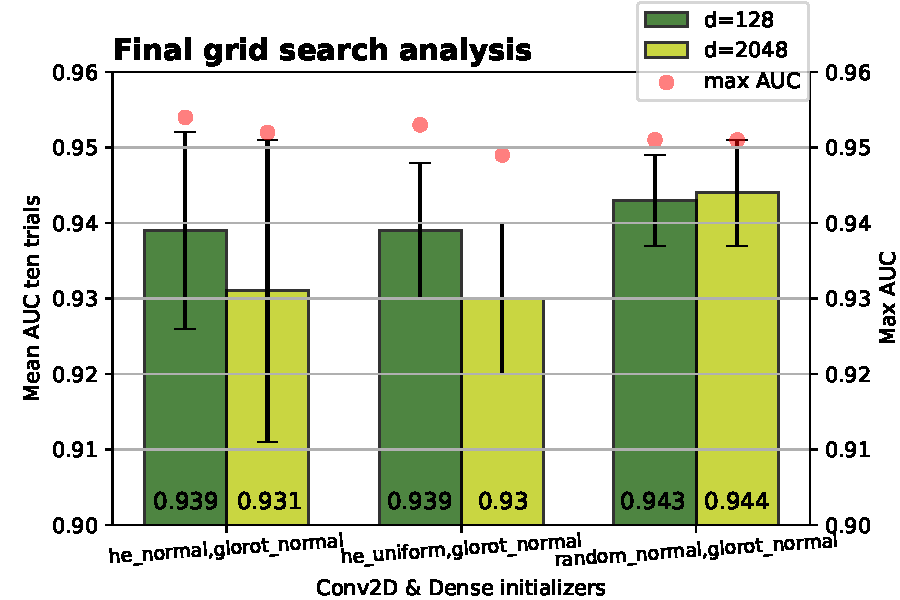
\includegraphics[height= 5cm]{images/contrastive/contrastive_loss_final_bar}
\caption{Final grid search analysis}
\label{fig:contrastive_loss_final_bar}
\end{figure}

\textbf{Conclusion}
The best result was obtained by RandomNormal and glorot normal as Conv2D and dense layer initializers respectively. Along with 128 and 2048 dense units values both resulting very close mean AUC values. So the best
result is mean AUC (Ten trials) of 0.944 with std of 0.007 and highest AUC value in a single run as 0.95. 

The state of the art is AUC of 0.91, so the finding in this work hints at slight improvement.
%\subsection{To finish the contrastive loss analysis}
%\begin{itemize}
% \item Network diagrams -- done
% \item Theory on contrastive loss
% \item Theory on Siamese
% \item Training process
% \item Explain the search space 
% \item Graphs -- Done
% \item Computation time and memory usage and computation power
% \item Adding the Search spaces into Appendix (Much later)
%\end{itemize}

